%\documentclass[]{article}
\documentclass{sig-alternate-05-2015}

%opening
\title{Analyzing the effect of "Majority is not Enough" on the Blockchain}
\numberofauthors{2}
\author{
\alignauthor
Lucas Chaufournier 
\alignauthor
Cassie Corey}

\begin{document}



\maketitle


\section{Introduction \& Motivation}
In November 2013, Eyal and Sirer published \textit{Majority is not
Enough: Bitcoin Mining is Vulnerable} which presented a new attack known as
Selfish Mining. They posited that it was no longer enough for an attacker
to have a majority of the mining power to attack the network and that
instead with as little as 1/3 of the mining power they can unfairly gain
blocks. 

They established that by secretly mining on a hidden fork and not releasing
blocks, they are able to get ahead of the main chain and as the main chain
catches up, they can selectively release blocks to maintain their lead.
Every time the main chain releases a block, the attacker can release two
blocks, one to match the viable block and one to orphan said viable block,
thus granting them the coinbase for both blocks. An Attacker can
theoretically perform this attack indefinitely or at the very least until the difficulty changes. 

Alongside this novel attack, they also disclosed
two theoretical telltale signs of a selfish mining attack, so that it may be detected
in the blockchain. The process of selfish mining requires that you
orphan legitimate blocks, thus there will inevitably be orphans in the
blockchain that can be used as a signal to investigate a portion of the blockchain. Further, since
selfish mining requires that you release multiple blocks at one time to
orphan the legitimate block, the timestamps between the blocks will be less
than the average 8 minutes of most blocks. By combining these two indicators, it should theoretically be possible to detect selfish mining on the blockchain. 

Our project aims to investigate the effect that the Selfish Mining paper had on the blockchain. We hypothesize that before the paper, selfish mining was a relatively unknown technique and had not been performed on the blockchain. Due to the wide recognition of this paper, we believe that selfish mining has been attempted and that it should be detectable on the blockchain. We set forth to analyze these hypothesis and to see what the probability is that certain sections in the blockchain could be actual selfish mining.  
\section{Related Work}
The current consensus is that no selfish mining has occurred on the blockchain as of yet. These analysis's were conducted using the two indicators that were previously mentioned: orphaned blocks \& timing of successive blocks. Unfortunately, there are some issues with these two methods as a means of indication. 

First, common sites that are used to scrape data from the blockchain misreport data on the number of orphaned blocks. From our analysis with blockchain.info, we were only able to see 817 orphaned blocks for the duration of bitcoin's lifespan. This is obviously incorrect and is likely due to numerous factors. Most likely, blockchain.info only keeps track of a single orphan or the latest orphan for a group of orphans on the blockchain. It is also hard for all nodes to keep track of orphans due to propagation delays and miners not wanting to propagate orphaned blocks outside their pools. With the lack of reliable orphan date, orphaned blocks become an unlikely and unreliable indicator of selfish mining.

Timing between blocks can also be an unreliable source of data. Timestamps are dictated by the miners releasing the announced block and any time is valid as long as it is greater than the median timestamp of the previous 11 blocks and less than the median of the timestamps returned by all nodes connected to the miner + 2 hours. Theoretically, a selfish miner could adjust the timestamps such that things appear normal on the blockchain. This can also lead to issues where block timestamps appear as if they are out of order when in fact the timestamps are just wrong. 

In our analysis, we ran into issues with both orphans and timestamps, which made it difficult to reliably analyze the data. We decided to ignore orphan blocks as an indicator as the data we had was too few and unreliable. We focused our efforts on examining timestamps, although still unreliable, with enough tuning we can get a rough approximation whether activity is suspicious. An issue we had to work through was that if miners can set their own timestamps, how do you decide what is a suspicious amount of time between blocks. We chose to examine chains of blocks for several thresholds but focus on those that are lengthy and small. We discuss this further in the section on methodology.
\section{Our Methodology}
\subsection{Gathering Data}
The blockchain, although portable, contains a non-insignificant amount of data and requires a fast connection to download. To save on time and storage space we analyze data from blockchain.info using their python api. Unfortunately, blockchain.info rate limits general users unless you have an api token and while we requested a key we did not hear back from them. To avoid being repeatedly blocked from their servers and to speed up the collection of enough blockchain data we used the api to make a request that grabs a list of simple blocks for a given day(\texttt{blockexplorer.get\_blocks}).

A simple block is a block that has no transactions rather it has just the height, hash, time and a boolean saying whether it is part of the main\_chain. This was more than enough data for our analysis. We were able to get a list of simple blocks for every days since the creation of bitcoin in a little under an hour. This list contains over 400,000 blocks. 

We then used the pickle library to write the list of blocks to a file so we only had to request the blockchain once. Once we acquired our blockchain, we then proceeded to calculate the times between blocks and save that to a file as well. This provided us with a list of timing data that we end up using for our analysis. 

Once we compiled our data, we divided the dataset into two smaller datasets. One dataset represents the timings of blocks between the genesis block and December 31st 2012 and the other represents the timings of blocks between January 1st, 2013 and April 2016. Both datasets are relatively equal in size with the before dataset consisting of 208,133 block timings while the after data set has 192,389 block timings. We chose January 1st as our boundary because that is roughly 11 months before the paper was published. This enables us to exclude work done on the blockchain during production of the paper from our before data set.


\subsection{Examining Data}
With our two data sets we first calculated the cumulative percent of block timings(the time between two blocks) that occur at a certain time period. If the time between blocks was under two minutes then that would be factored into the percentage of block times under 2 minutes. Figures 1, 2 and 3 represent the cumulative graphs for Before the paper, After the Paper, and Overall. 

We next computed chains that appear in the blockchain. A chain represents timings between blocks that are in successive order and all appear within a certain threshold of each other. If the timing of blocks is 8,1,1.2,1.3,1.05,9 then a chain would be produced from this set that looks like [1,1.2,1.3,1.05] because these data points are in a row and are all within 1 minute of each other. We compute chains by iterating over the timing data, and setting a marker equal to the current block. We then append the current block to a new list. On the next item we examine if it is within a threshold of 1 minute of the current marker, if so append to the current list. If not we save the current list, set the marker to the current item and then append it to its own new list. We repeat this process throughout the entire blockchain dataset so that we can examine runs that appear in the blockchain. 

An important note is that these chains represent the upper bound so even though a chain of 5 also represents chains of 4 and 3 and 2 and 1 we ignore these chains. We can also produce longer chains by increasing threshold so that it accepts items that are greater than 1 minute from the marker. If we are interested in chains that have differences of 3 minutes or less, it can be tuned to produce these longer chains. We decide to focus on chains that represent smaller durations.    

With our new chains, we examined the frequency of occurrence in the blockchain data sets. Figures 4 and 5 represent histograms for chains where there was only 1 minute difference among the blocks in said chain for the data sets before and after the paper.

We also sought to calculate the chance that any chain of length n for a given time threshold x and total blocks z could naturally occur in the block chain. We derive a formula as follows. The probability that a block occurs with a time of t since the last block is given from the probability distribution that is demonstrated in figures 3, 4 and 5. From the figures there is a roughly 10\% chance that the time between two blocks is 1 minute or less. Using this probability we can calculate what the chance that the following chain occurs naturally: [..,1,.56,.34,.47,.12,...]. We first calculate the probability of it happening once: x=10\%. Now to calculate n=4 blocks in a row you need to multiply: \(.1*.1*.1*.1\) otherwise known as \(.1^4\). This is the probability that this chain has occurred. Now we calculate the chance that this does not occur at all naturally by calculating: \(1-.1^4\). Now we choose to calculate the chance this does not occur for \(z=400,000\) blocks: \((1-.1^4)^{400000}\). Finally, to calculate the overall probability that this occurs at least once we just take the result from 1:  \(1-(1-.1^4)^{400000}\). This results in a value of: 1, that is there is a 100\% chance that this occurs naturally. We present a more generic formula that can be used for further analysis below: \[1-(1-x^n)^{z}\]  where x is the probability of said time occurring, n is the number of blocks in a row, and z is the total number of blocks. In the following section we dig deeper to see what the properties of a chain would have to become suspicious.
\begin{figure}
\centering
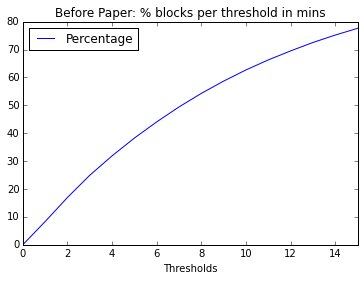
\includegraphics[height=2.5in, width=3in]{before.png}
\caption{ Percent of block timings before the paper under a certain threshold t}
\end{figure}

\begin{figure}
\centering
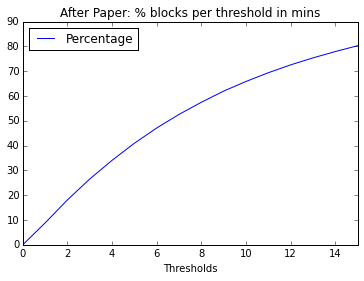
\includegraphics[height=2.5in, width=3in]{after.png}
\caption{ Percent of block timings after the paper under a certain threshold t}
\end{figure}


\begin{figure}
\centering
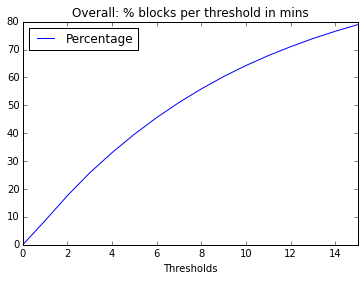
\includegraphics[height=2.5in, width=3in]{overall.png}
\caption{ Overall Percent of block timings under a certain threshold t}
\end{figure}

\begin{figure}
\centering
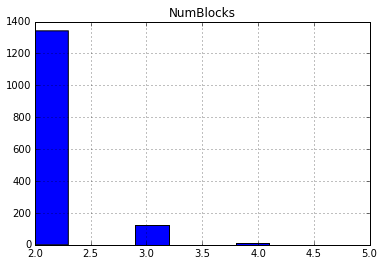
\includegraphics[height=2.5in, width=3in]{before_one_dist.png}
\caption{ Before Paper: Distribution of chains of 1 minute difference in time between blocks}
\end{figure}


\begin{figure}
\centering
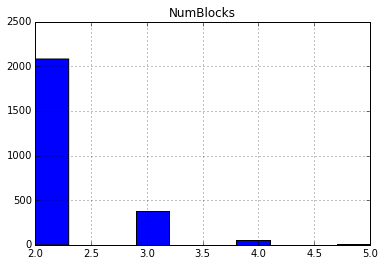
\includegraphics[height=2.5in, width=3in]{after_one_dist.png}
\caption{ After Paper: Distribution of chains of 1 minute difference in time between blocks}
\end{figure}




\section{Results \& Evaluation}
We now seek to examine a little closer and reflect on our findings. We first examine our findings on the distribution of timing between blocks to see how the paper affected things. We then proceed to examine the distribution for timing chains that occur in the blockchain and their rate of occurrence. We then conclude with what it would take for a chain of blocks to be of a non-natural length.  


\subsection{Distribution of Block Timings}
The distribution of Block Timings for before and after the selfish mining paper and the overall blockchain are presented in Figures 1, 2 and 3. Before the paper, our data shows the expected results of timing distribution with a low percentage around the 1, 2 and 3 time lengths and a majority over the 8 minute mark. If you were to choose two blocks from the blockchain there is a roughly 55\% chance of the blocks being 8 minutes or less apart. 

After the paper was published, the data shifts a little but not a significant enough amount to declare that the paper had any effect on the distribution. The majority still hangs around 8 minutes or lower but the percentage of longer times between blocks seems to have decreased. This is likely due to the fact that their are less blocks and we no longer include in the dataset the originally mined blocks where there could be 2 days between blocks. This indicates this dataset is a more realistic distribution due to the lack of extreme outliers.

We conclude that based merely on the overall distributions of block timings, the paper had no effect. It is important to mention that this does not necessarily indicate no selfish mining has occurred. It could simply be that selfish mining was discovered early on and not revealed until the paper was published. If this were the case you would expect little to no change in the distribution. This is a highly unlikely result and impossible to verify but should not be entirely ignored. We next proceed to examine how the paper affected the length of chains in the blockchain. 

\subsection{Distribution of Chains}
In figures 4 and 5, we present the distribution of chains where the members of said chains are a minute or less, i.e [1,.5,1,.99,.45] for before and after the paper. In figure 4, a majority of the chains are of length 2 while only a few hundred are length 3 and maybe 20 or less are length 4. In figure 5, we see a similar result, but we can see that chains of length 3 have nearly doubled and chains of length 4 are still few but more significant. 

It is expected that, with this many blocks being examined, we would find thousands of chains of length 2 that are a minute apart. This is a result of basic chance and thus it is safe to ignore chains of length 2. More attention should instead be paid to the tail ends of the distribution as that is where suspicious behavior is likely to be found. It is interesting to see that after the paper was published the number of chains length 3 and 4 did increase. Whether this is due to the paper or decreases in puzzle difficulty is difficult to verify, and we should be careful of "Correlation does not imply causation". At least there is a place to start looking in future work to investigate if selfish mining is occurring at these points. 

\subsection{What are the chances?}
We mentioned earlier that the probability of a chain of length n occurring for a given chance x in z total blocks is \[1-(1-x^n)^{z}\]. For most small n's this will be close to if not 1, which is to be expected when dealing with larger exponents. We are going to take a closer look and see how many blocks in a row it would take to produce a chain of a non-natural length for a threshold of two minutes or less. The chances of a block being two minutes or less is around 15\% as seen in Figure 3. 

In figure 6, you can see our probability formula plotted against various chain lengths using an x value of .15 for 2 minutes or less between blocks. As you can see for chains of length 0-7 there is almost 100\% probability of them naturally occurring in the blockchain. When you hit chains of 8 blocks, the chances of said chain occurring naturally starts to decrease. At chain lengths of 8 blocks with each block in the chain being 2 mins or less apart, the chances of occurring is a little less than 10\%. At lengths of 9, there is a 1\% chance and at length of 10, there is a less than 1\% chance for a chain. We can then compute these for the all values of x and n and compare against the blockchain to locate any suspicious length chains. This is beyond the scope of this project as we chose to focus on a small proof of concept. 

We did examine the blockchain for chains of 2 minutes or less and the longest chain we could find was of length 4, well within the realm of natural occurrence. For blocks of less than 1 minute, the longest chain we found was of length 4 which is also within in the realm of natural occurrence.     



\section{Conclusion}
Overall we can not definitively say how the selfish mining paper affected the blockchain. It appears as if the paper had a minimal effect on the blockchain and a slight increase on the number of chains of length 3 and 4, though we can not definitively conclude that was the caused by the paper. We calculated the probability of a chain of n length for z total blocks occurring naturally and we saw what values of length n would push us into the realm of non-naturalness. We also verified this against the blockchain to see if unnatural values occurred but more in depth analysis is needed to say for sure if there are suspicious chains.   

\section{References}
1. Majority is not Enough: Bitcoin Mining is Vulnerable, Ittay Eyal and Emin Gun Sirer, 2013, http://arxiv.org/abs/1311.0243 

2. Bitcoin Wiki, Block Timestamp, 2016, https://en.bitcoin.it/wiki
/Block\_timestamp

\begin{figure}
	\centering
	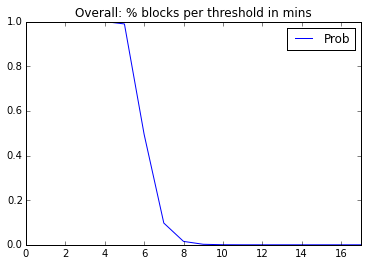
\includegraphics[height=2.5in, width=3in]{probability.png}
	\caption{ Chances of a chain length x for 400,000 blocks given a distribution of 15\% for timings of length 2 minutes or less.}
\end{figure} 
\end{document}
